\newpage
\subsubsection{\large\hei {乌龙院~{\small 之}~宋江}}
\addcontentsline{toc}{subsection}{\hei 乌龙院~{\small 之}~松江}

\hangafter=1                   %2. 设置从第1⾏之后开始悬挂缩进  %}
\setlength{\parindent}{0pt}{

{\vspace{3pt}{\centerline{{[}{\hei 第一场}{]}}}\vspace{5pt}}

{列位,少陪了!}

\setlength{\hangindent}{56pt}{【{\akai 四平调}】大堂上打罢(了)退堂鼓,衙前来了宋公{\footnotesize 呃}明。}

{卑人宋江,在这郓城县中,当了一名刑房书吏。今日太爷退堂甚早,房中无事,多日未到乌龙院中,不免前去走走。}

\setlength{\hangindent}{56pt}{【{\akai 四平调}】那一日闲游长街上,遇着好汉叫刘唐。他把那实情事对我讲,请我到梁山去为王。富贵岂容人妄想,自有天爷作主张。}

\setlength{\hangindent}{56pt}{【{\akai 四平调}】一步儿}\footnote{``一步儿''原记作``移步儿'',从吴小如先生建议改。}{来在大街上,}

\setlength{\hangindent}{56pt}{(搭架子\hspace{18pt}({\akai 内})$\cdots{}\cdots{}$老丈诶,嘿嘿嘿,$\cdots{}\cdots{}$同走一条道路$\cdots{}\cdots{}$可笑$\cdots{}\cdots{}$哈哈哈$\cdots{}\cdots{}$({\hwfs 笑介}))}

{啊!}

\setlength{\hangindent}{56pt}{【{\akai 四平调}】又听得众人说短道长。}

{耳旁听得众人议论({\akai 或}:~谈论)。嗯,待我问来。}

{列位,请了!}

{借问一声,方才大家议论何事?}

{哦,衙中有事,改日(再来)讨扰。}

{哎呀且住,方才分明听得众人言讲:~``前面走的张文远,后面跟随宋公明。师徒二人,同走一条道路$\cdots{}\cdots{}$''({\hwfs 惊介})莫非张文远这小奴才({\akai 或}:~这个奴才),也往乌龙院中行走不成?}

{哎呀,({\akai 念})是非终朝有,不信自然无。}

\setlength{\hangindent}{56pt}{【{\akai 四平调}】好话出在君子口,立志不听这小人言。}

\setlength{\hangindent}{56pt}{【{\akai 四平调}】一步儿来在乌龙院,}

{啊?!}

\setlength{\hangindent}{56pt}{【{\akai 四平调}】青天白日把门关。}

{啊?为何将院门关闭了?}

{嗯,待我叫门。}

{啊,大姐开门来。}

{大姐,开门来。}

{呔,开门来呀!}

{是我啊!}

{怎么连宋大爷的声音都听不出来了?}

{诶,开门!}

{钥匙今在何处?}

{诶,快些取来。}

{为何这样慢腾腾的?}

{待我闯了进去呀。}

{\textless{}\!{\bfseries\akai 哭皇天}\!\textgreater{}啊$\cdots{}\cdots{}$}

{往日宋大爷到此,地面清洁,画幅高悬。今日进得院来,(这)地也未曾扫,画也不曾挂。呃,幸喜(是)你宋大爷一人前来呀,倘有朋友同来,成何体统啊?}

{哦,这也难怪呀。}

{诶,大姐,这就是你的不是了:~宋大爷到来,就该搬个座位,让你宋大爷坐下的才是啊。你一人,大模大样,坐在一旁。诶,岂不是轻慢你宋大爷,呃,小看你,呃,宋大爷么?(呃,真真的岂有此理呀!)}

{是啊({\akai 或}:~哦)。(都是)自家的东西,有的是座位,呃,何劳大姐来动手{\footnotesize 哇}。}

{家无常礼。}

{\textless{}\!{\bfseries\akai 哭皇天}\!\textgreater{}自家的椅儿自家搬{\footnotesize 呃}$\cdots{}\cdots{}$}

{啊大姐,你好啊?}

{我也好。}

{呃,我问过大姐,大姐自然要来问我啊。我便说了({\akai 或}:~先说了),免得有劳大姐的精气神{\footnotesize 呐}。}

{\textless{}\!{\bfseries\akai 哭皇天}\!\textgreater{}啊$\cdots{}\cdots{}$}

{嗯嗯,这是尊敬大姐。}

{啊}大姐,你可喜欢这个调调儿?

{嗯嗯嗯,我们就免去这个调调儿。}

{请坐。}

{啊大姐,你手拿何物啊?}

{诶,分明是一只红绣花鞋,怎说是卑人的帽儿呢?}

{呵,这是哪个穿的?}

{诶,妈儿娘偌大的年纪,怎么还穿这样的红绣花鞋呀?}

{哎呀,不好啊。}

{哦哦哦,不是大姐提起,卑人就({\akai 或}:~卑人倒)忘怀了。明日我是礼到人也到。}

{一定要来!}

{呃,一定要来。}

{呃,呃,呃,大姐,闻得(大姐)一双巧手,做得好活计,嗯,今日我要瞻仰瞻仰。}

{呃,一定要瞻仰(瞻仰)。}

{哦,哦,哦,是是是,适才在衙中,抄写文卷,玷染了双手,嗯,待我来擦上一擦,擦上一擦。}

{干净了。}

{啊,大姐你看我如何啊?呵呵$\cdots{}\cdots{}$({\hwfs 陪笑介})}

{啊?!你道({\akai 或}:~你嫌)我双手不洁,如今将鞋抛在地上,难道这地面就干净么?这是怎样啊?!}

{哼,你怎么就这样不讲道理啊。}

{哼,不讲道理啊!}

{是啊,``洗手净指甲,着鞋泥里踏。''终究是要脏的呀。}

{呃,是这只$\cdots{}\cdots{}$鞋儿啊。}

{呃,待我来(瞻仰瞻仰,)看上一看。}

{好!}

{人生天地之间,哪里有不知好歹的道理呀?}

{好,好,好。}

{呃------({\hwfs 思索介})花儿好,样儿好,做得好,这就是好,好,好({\akai 或}:~嗯------好,好,好)!}

{嗯------还有什么褒贬么? ({\hwfs 思索介})}

{这就是它的颜色不正。}

{呃,(乃是)这只$\cdots{}\cdots{}$鞋呀。}

{啊大姐,我看你神色不快呀,莫非有什么心事不成么?}

{慢说大姐的心事,就是我家太爷的心事,卑人不猜便罢------}

{嗯,(我)一定要猜他个八九不离十。}

{今日无事,呃,我一定要猜上一猜。}

{呃,(我)一定要猜。}

{(大姐)听了------}

\setlength{\hangindent}{56pt}{【{\akai 四平调}】宋公明打坐乌龙院,猜一猜大姐腹内情。莫不是茶饭不对你的口,}

{呃,不是的?再听呐!}

\setlength{\hangindent}{56pt}{【{\akai 四平调}】莫不是衣衫不合你的身?}

{呃,也不是的。嗯,是的------}

\setlength{\hangindent}{56pt}{【{\akai 四平调}】莫不是邻居们得罪了你,}

{嗯,你说的是啊。哦,哦,哦,是了!}

\setlength{\hangindent}{56pt}{【{\akai 四平调}】莫不是妈儿娘打骂不仁。}

{呃,这倒难猜了!}

\setlength{\hangindent}{56pt}{【{\akai 四平调}】这不是来那不是,}

{啊大姐,我这一下就一定猜着了!}

{大姐(听了)------}

\setlength{\hangindent}{56pt}{【{\akai 四平调}】莫不是思想我宋公明。}

{(看)我猜着了吧?}

{哼,你是想我?}

{你想我,你是怎样的想法呢({\akai 或}:~怎样想我啊)?}

{呃,呃,衙中有事啊。}

{昨天------哦,与朋友吃酒。}

{今日------我可就来了哇。}

{怎样的厉害?({\akai 或}:~哦,你是怎样,怎样的,怎样的厉害?)}

{哎呀,这是什么想法啊?}

{这,凉水,}

{这,蒜$\cdots{}\cdots{}$蒜?}

{这是淡思淡想}\footnote{``淡思淡想'',即``单思单想''的谐音。}{啊!}

{嗯,大姐,你不是想我吧?}

{哪个想我啊?}

{呀呸!}

\setlength{\hangindent}{56pt}{【{\akai 二黄摇板}】适才听得人议论,言语恍惚事不明。话到舌尖留半句,说出口来你难为人。}

{嗯,}

{这二,}

{这三------}

{三$\cdots{}\cdots{}$}

{唉,就是这个三呐$\cdots{}\cdots{}$}

\setlength{\hangindent}{56pt}{【{\akai 二黄摇板}】都说你私通了({\akai 或}:~私通那)张$\cdots{}\cdots{}$\textless{}\!{\bfseries\akai 行弦}\!\textgreater{}}

{唉!}

\setlength{\hangindent}{56pt}{【{\akai 二黄摇板}】都说你私通了张文远。}

{是个姓张的。}

{哪个三?({\akai 或}:~三------三$\cdots{}\cdots{}$)}

{哼,你的心事我还能猜不着?}

{姓张的呀!}

{呀呸!街前街后,哪个不叫我宋大爷,偏偏要你来叫?(哼!)}

{呀呸!衙里衙外,哪个不叫我宋先生,要你来奉承?哼!}

{哦,怎么,你吃了酒了?}

{酒后言多语失啊!}

{诶,今后少饮些也就是了。}

{呃,他们说有个姓张的,}

{(就)是那(个)张文远呐,你是晓得的呀。}

{他是我的徒儿啊。({\akai 或}:~诶,那张文远,他是我的徒儿啊。)}

{同在刑房,抄写文卷。}

{同宿值夜,抵足而眠。}

{呃,房漏了?找房东啊。}

{诶,哪有这样的事(体)啊?!}

{(是)哪个?}

{住口!}

\setlength{\hangindent}{56pt}{【{\akai 西皮导板}】一言怒恼宋公明,}

{阎大姐!}

{阎惜姣!}

{呵呵,你叫起你宋大爷的官印来了!}

{我$\cdots{}\cdots{}$我把你这个贼淫妇哇!}

{唉,想我宋江花费多少的精神,倒落了一个``无耻''之名喏!}

\setlength{\hangindent}{56pt}{【{\akai 西皮原板}】骂一声阎惜姣无义贱人。曾记得那年遭荒旱,你一家三人来到郓城。买你的身价三十两,我为你得罪了【{\footnotesize 转}{\akai 西皮快板}】众家的宾朋。我为你造了({\akai 或}:~建了)乌龙院,我为你花费许多银。我为你【{\footnotesize 转}{\akai 西皮摇板}】在父母台前不能够行孝,}

{呀呸!}

\setlength{\hangindent}{56pt}{【{\akai 西皮快板}】我为你拆散夫妻情。一怒赶出乌龙院。}

\setlength{\hangindent}{56pt}{【{\akai 西皮摇板}】任你逃至天涯外,难逃宋江的掌握中。}

{(我料得定!)}

{(我)料得定!}

{呀呸!}

\setlength{\hangindent}{56pt}{【{\akai 西皮摇板}】两鬓蓬松贼淫妇,水性杨花下贱人。恨不得举拳将你打,\textless{}\!{\bfseries\akai 行弦}\!\textgreater{}}

{哼!}

\setlength{\hangindent}{56pt}{【{\akai 西皮摇板}】大丈夫打妻不算人。从今后不进乌龙院,敢对苍天把誓盟。}

{呃,呃,唉------大姐,卑人今早也是吃了早酒了,言语不逊,呃,莫要计较啊({\akai 或}:~你不要计较啊)!}

{哎呀!}

\setlength{\hangindent}{56pt}{【{\akai 西皮摇板}】宋江跪在地埃尘,过往神灵听分明:~我若再进乌龙院,药酒毒死我宋公明。}

{诶呀,夫妇争论几句,何须当真({\akai 或}:~何必认真)。待我回去。}

{啊?!这贱人竟将院门关闭了({\akai 或}:~竟将门户关闭了)!}

{唉------呀!}

{({\akai 念})当初不听朋友劝,失足上了无底船。受了许多肮脏气,花了许多昧心钱。}

{唉,大丈夫拾得起,放得下!}

{说不来,我就不来了!}

{呃,待我走去!}

{唉呀!说什么不来,说什么走去!}

{想这乌龙院乃(是)我宋江亲身所建}({\akai 或}:~亲自所建){,我若不来,看你们哪一个大胆的敢来?!}

{从今以后,这乌龙院中无事便罢,倘有风吹草动,嗯!我就是这一刀------}

{(宋江用扇子比势)}

{定要结果尔的狗命!}

{你要仔细了,你要打点了!}

{唉,(我)再也不来了。}

{\vspace{3pt}{\centerline{{[}{\hei 第二场}{]}}}\vspace{5pt}}

{呃,妈儿娘,呃,今日衙中有事,呃,改日再会。}

{呃,大街之上拉拉扯扯,成何体统啊?}

{你放手,我随你前去就是。}

{唉!}

{呃,告辞了。}

{她不是想我!}

{(她)说的不是我啊!}

{要去。你去,我不去!}

{呃,告辞了!}

{呃,呃,外面不要上门锁。({\akai 或}:~外面不要上门啊。)}

{(阎婆

里面不要上门闩。)}

{(不要加锁啊。)}

{呃,我明日早衙(还)有事啊!}

{大姐,惜娇!}

{她径自一人睡去了!}

{唉,想我宋江,英雄当世,今晚再宿乌龙院中,好不悔闷人也!}

\setlength{\hangindent}{56pt}{【{\akai 四平调}】一更紧催一更尽,秋气透窗伴孤灯。她先前待我情义重,为何今日变了心,啊,变了心。}

\setlength{\hangindent}{56pt}{【{\akai 四平调}】玉漏迢迢银河耿,仗义英雄\footnote{樊剑{\scriptsize 君}告,刘曾复先生授其作``斜月透窗''。}气似虹。直饶如今才知悔,何不当初莫来行,啊,莫来行。}

{妈儿娘,(妈儿娘,)开门来!}

{开门来!}

{呃!({\akai 念})有事在心头,终日愁眉皱。}

{走啊!}

{哎呀且住!只顾行走,不想将招文袋失却。}

{想这袋中,虽有黄金一锭,并无妨碍,只有那封书信,事关紧要,一旦泄漏,如何得了!}

{哎呀!(这这这$\cdots{}\cdots{}$)}

{唉!事到如今,也只得再次进院了!}

{罢!}

{啊,大姐醒来,大姐醒来!}

{呃,是我又回来了哇。}

正是,呃呃,不错!

就是那个袋儿。

唉,旁人背地闲言碎语,今日显出这样的善良之心,真真的({\akai 或}:~真真是)难得呀!

{啊,大姐可曾看见这袋内的金锭({\akai 或}:~黄金){\footnotesize 呐}?}

{呃,原是要交与大姐(你)的。}

{呃,这里面------}

{呃,不错,正是一封书信。({\akai 或}:~呃,不错不错不错,正是,里面有一封书信。)}

{呃,呃,乃是故友来信{\footnotesize 呐}。({\akai 或}:~乃是朋友的书信{\footnotesize 呐}。)}

{(是)什么?}

{大姐你噤声!}

{你莫要高声呐!}

{大姐,(把信)还与卑人罢!}

{念在你我夫妻一场({\akai 或}:~念在你我从先的恩爱),把还我罢!({\akai 或}:~把我罢。)}

{(把我罢。)}

{(还我罢。)}

{依你什么?}

{呃呃,(我)依得依得!}

{何谓``了断''?}

{诶,你无``七条''之犯,休书如何写得?}

{不能写呀。}

{哪里去?}

{呃,好,好,好,我写我写。}

{呃,还是不能写啊。}

{无有文房四宝,怎样写得呀。}

{哦------原来你早有此意么?!唉!}

{唉!待我来写。}

{我是怎样写呀?}

{罢!你讲我写!}

{妾!}

{妾与妻大不相同({\akai 或}:~大有不同)。}

{就任凭你改嫁------}

{诶,你改嫁别人,任凭于你,单单就是不容你嫁那个姓张的!}

{我$\cdots{}\cdots{}$不写!}

{哪里去?}

{慢来(慢来)!}

{罢!(我)就任凭你改嫁那张文远!}

{拿去!}

{为何?}

{哦------还要打(上)手模足印\footnote{``手模足印''刘曾复先生认为应作``手模指印''。据《老结婚证书》\upcite{Marry}载,现存辽宁省档案馆明嘉靖年间的婚书上面的脚印清晰完整(婚书为素黄宣纸书写,因年代久远,婚书和上诉的状纸均已残缺)。2022年,微博网友提供的光绪十八年立的休书也有完整的手模足印(附后),故从之。}么?!}

{(不能打!)}

{我不卖妻,打的什么手模足印?!}

{我不能打!}

{回来,我就与你打!}

{这是哪个教({\akai 或}:~教导于)你的?}

{哼!拿去。}

{且慢,要两下交换。}

{(两下交换。)}

{好,就依你(之见),拿去。}

{回来!(呃,你还我那书信呐?)}

{我件件依你,你怎么还不还与我的书信呐?}

{你快快(地)还我!}

{哪里还我?}

{啊?!这郓城县大堂是狼?}

{是虎?}

{还吞吃我宋江不成?!}

{啊,阎大姐呀!还望念在从先的一点点的情分,把书信还我罢!}

{我求你------把信还我罢!}

{你不要再三地逼迫了!}

{你,你,你不要逼出事来呀!}

{我$\cdots{}\cdots{}$我不骂你,}

{我$\cdots{}\cdots{}$不打你。}

{我$\cdots{}\cdots{}$我$\cdots{}\cdots{}$我不敢杀你$\cdots{}\cdots{}$}

{看刀!!}

{妈儿娘快来!}

{你的女儿------唉,我把她杀了!}

{哪个唬你?!}

{随我来呃!}

{诶------我不准你哭!}

{(我不准你嚎!)}

{你要哭,我也就要杀了你({\akai 或}:~我就也杀了你)!}

{呃,拿这锭金子({\akai 或}:~银子)去买。}

{随我去长街去抬啊。}

{噤声!}

{噤声!}

{噤声$\cdots{}\cdots{}$}

}
\vskip 15pt 
{\hei {\large 附:~{清光绪十八年的休书}}}

\begin{figure}[h!]
\centering
%\vspace{+0.2in}
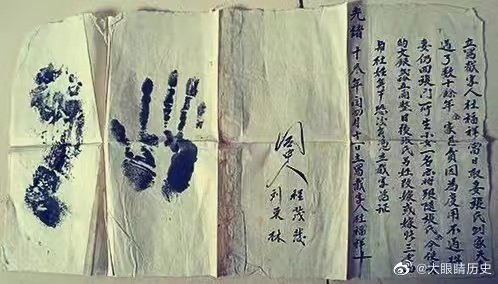
\includegraphics[height=0.36\textwidth,width=0.56\textwidth,viewport=0 0 375 240,clip]{Hand_and_foot-print.png}
\caption*{\hei 微博网页提供的清代光绪十八年~(公元1892年)~的休书} 
\label{Collect_Liu_Wu} 
\end{figure}

%\includegraphics{.jpeg}
\vskip 5pt

立写截字人杜福祥

当日娶妻张氏到家,夫妻过了数十余年。余家甚贫,因为度用不过,将妻仍回张门,所生小女一名,亦将跟随张氏。余今休妻的(得)文银贰拾伍两整,日后张氏另姓改嫁,或嫁张三、李四,与杜姓无干。恐说无凭,立截字为证。

\begin{flushright}
光绪十八年~闰四月十一日~立写截字人~~杜福祥 ~~(画 ``十字押'') ~~~\\
\large{同中人~程茂发、刘秉林} ~~~~~~~~~~ \\
\huge{手模}~~\huge{足印} ~~~~~~~
\end{flushright}
